\documentclass[14pt]{extreport}
\usepackage{gost}
\usepackage{tikz}
\usepackage{listings}
\usetikzlibrary{shapes.geometric}
\begin{document}
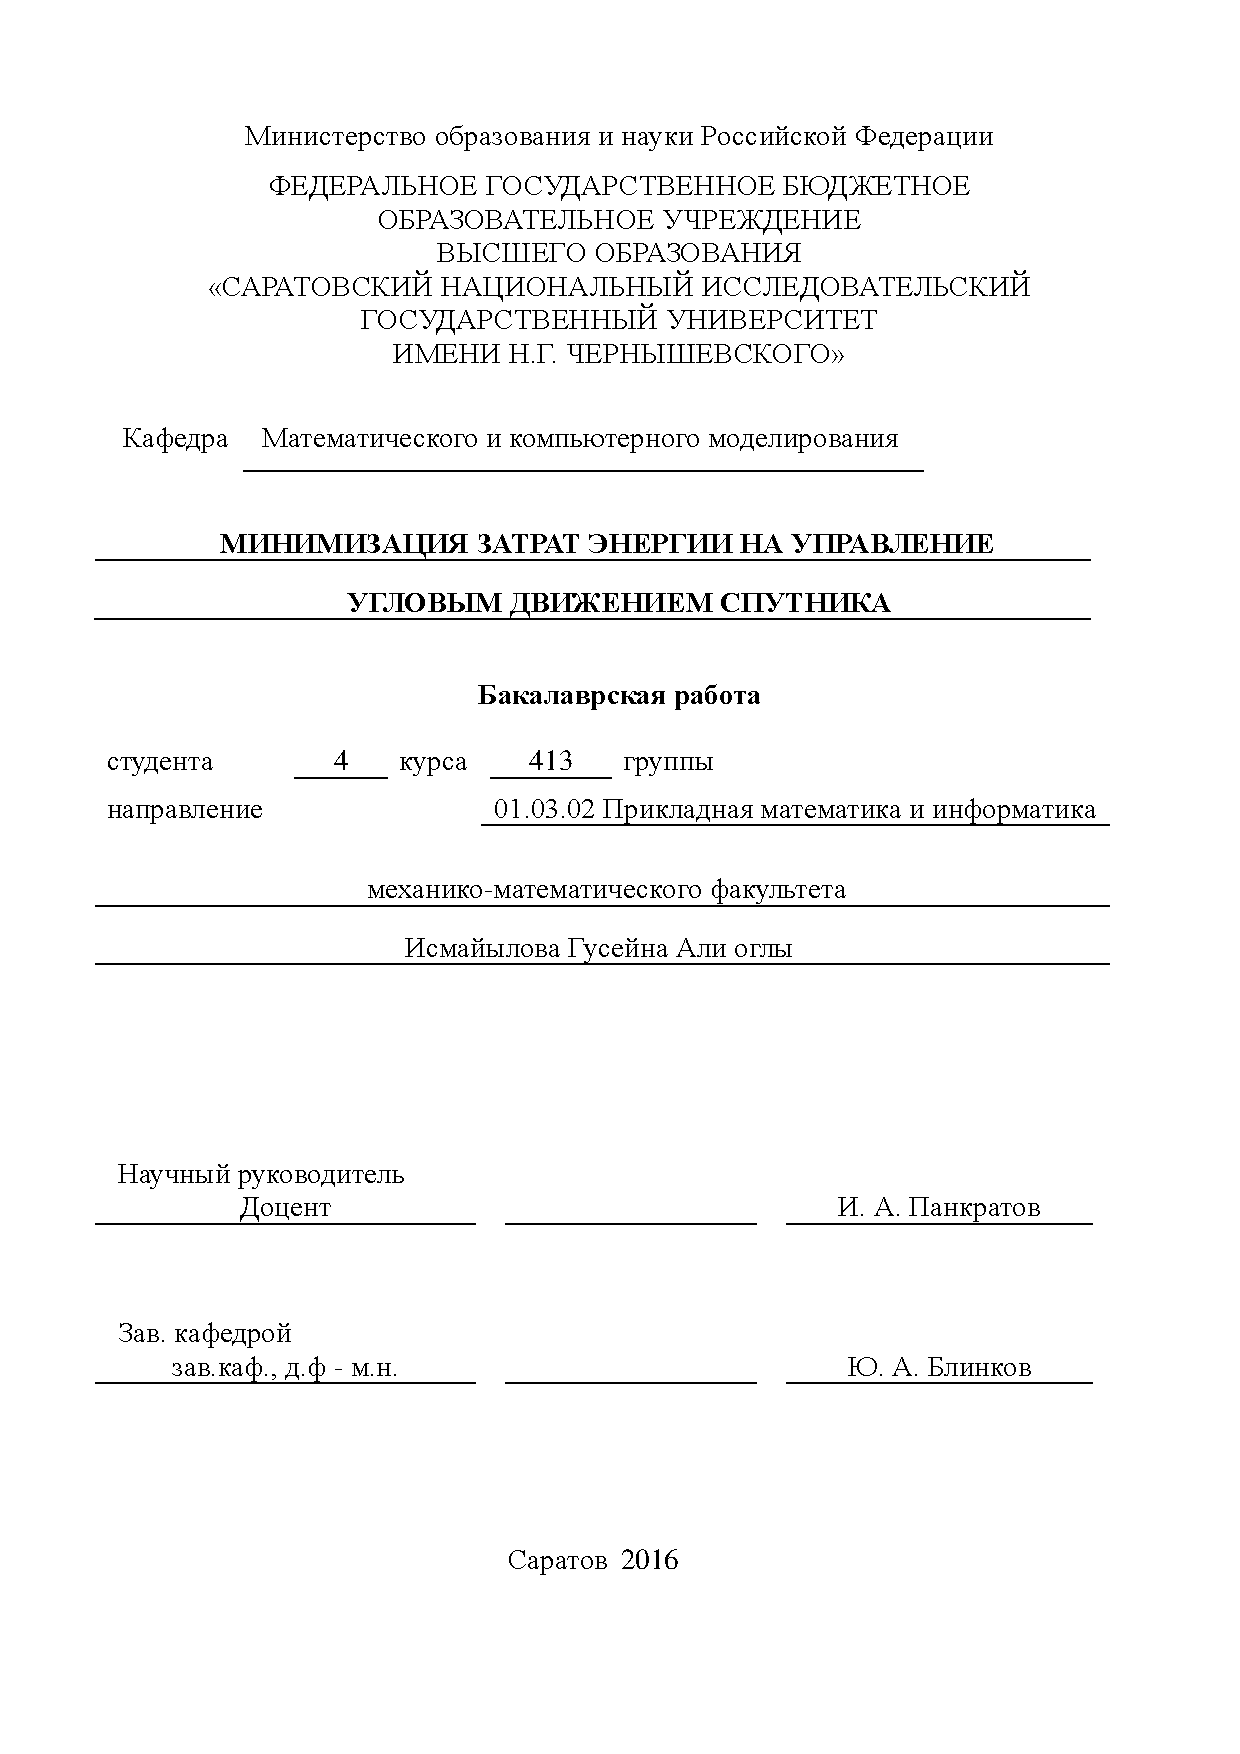
\includepdf[pages={1}]{titulDiplom.pdf}

\tableofcontents

\intro

Целью данной работы является ознакомление с методом конечных эле-
ментов, решение дифференциального уравнения на отрезке с граничными
условиями типа Дирихле и типа Неймана, нахождение значения интеграла
разбиением области на треугольники.

\chapter{Задача 1}
\section{ Постановка задачи и аналитическое решение}
Рассмотрим уравнение

Требуется решить следующее уравнение:
\begin{equation*}\frac{\mathrm{d}^2\varphi}{\mathrm{d}x^2} + \alpha\frac{\mathrm{d}\varphi}{dx} + \beta\varphi = 0,\eqno(1.1)\end{equation*}
где $\varphi$ -- неизвестная функция, методом конечных элементов на отрезке $[0, 1]$, рассмотреть случаи, когда краевые условия, имеющие вид
\begin{equation*}\begin{cases}1)\ \varphi(0) = 0,\ \varphi(1) = 1,\\ 2)\ \varphi(0) = 0,\ \frac{\mathrm{d}\varphi}{\mathrm{d}x}\bigg{|}_{x = 1} = 0,\end{cases}\eqno(1.2)\end{equation*} где $1)$ -- краевые условия типа Дирихле, $2)$ -- краевые условия типа Неймана.

Для начала найдем аналитическое решение задачи при $\alpha = -6,\ \beta = 9$.
Общее решение имеет вид: $\varphi(x) = c_1e^{3x} + c_2xe^{3x}$;

$1)$ Решение в случае с краевыми условиями типа Дирихле выглядит следующим образом: $\varphi(x) =e^{3x - 3}x$;

$2)$ Решение в случае с краевыми условиями типа Неймана выглядит следующим образом: $\varphi(x) =\frac{e^{3x - 3}x}{4}$\ .

\newpage

\section{Решение уравнения с помощью метода конечных элементов}
Рассмотрим общий вид нашей задачи:
\begin{equation*}
\begin{cases}
L\varphi+p=0, \varphi\in\Lambda, \\
T\varphi+r=0, \varphi\in\Gamma,
\end{cases}
\end{equation*}
где $L ~-$ линейный дифференциальный оператор и $T ~-$ линейный оператор, $p, r ~-$ не зависят от неизвестной функции.

Решение будем искать в виде $\widetilde{\varphi}=\sum\limits_{k=1}^{M+1}\widetilde{\varphi}_kN_k$, где \begin{equation*}
N_k = 
\begin{cases}
0, & x \leq x_{k-1},\\
\dfrac{x-x_{k-1}}{x_{k}-x_{k-1}}, & x_{k-1}<x<x_{k},\\
1, & x=x_k,\\
\dfrac{x_{k+1}-x}{x_{k+1}-x_k}, & k_k<x<x_{k+1},\\
0, & x \geq x_{k+1}.
\end{cases}
\end{equation*}

а) Составим невязку: $R_\Lambda=L\widetilde{\varphi}+p$. Для того чтобы выполнялось $R_\Lambda\approx0$ потребуем $\int\limits_{\Lambda}R_\Lambda N_sd\Lambda=0$, то есть $\int\limits_{\Lambda}[L\widetilde{\varphi}+p] N_sd\Lambda=\int\limits_0^1\left[\dfrac{d^2\widetilde{\varphi}}{dx^2}\alpha\dfrac{d\widetilde{\varphi}}{dx}+\beta\widetilde{\varphi}\right]N_sdx=\int\limits_0^1\dfrac{d^2\widetilde{\varphi}}{dx^2}N_sdx+\int\limits_0^1\left[\alpha\dfrac{d\widetilde{\varphi}}{dx}+\beta\widetilde{\varphi}\right]N_sdx=0,\ s=\overline{1,\ M+1}$. Проинтегрируем первый интеграл по частям и подставим в полученное выражение: $$\int\limits_0^1\dfrac{d^2\widetilde{\varphi}}{dx^2}N_sdx+\int\limits_0^1\left[\alpha\dfrac{d\widetilde{\varphi}}{dx}+\beta\widetilde{\varphi}\right]N_sdx=$$
$$=\left.\left[\dfrac{d\widetilde{\varphi}}{dx}N_s\right]\right|_0^1-\int\limits_0^1\dfrac{d\widetilde{\varphi}}{dx}\dfrac{dN_s}{dx}dx+\int\limits_0^1\left[\alpha\dfrac{d\widetilde{\varphi}}{dx}+\beta\widetilde{\varphi}\right]N_sdx=0,$$
$$\int\limits_0^1\left[-\dfrac{d\widetilde{\varphi}}{dx}\dfrac{dN_s}{dx}\alpha\dfrac{d\widetilde{\varphi}}{dx}N_s+\beta\widetilde{\varphi}N_s\right]dx=-\left.\left[\dfrac{d\widetilde{\varphi}}{dx}N_s\right]\right|_0^1,\ s=\overline{1,\ M+1}.$$

Получили СЛАУ $\sum\limits_{k=1}^{M+1}K_{sk}\widetilde{\varphi}_k=f_s, \ s=\overline{1,\ M+1},$ где $$K_{sk}=\int\limits_0^1\left[-\dfrac{dN_k}{dx}\dfrac{dN_s}{dx}\alpha\dfrac{dN_k}{dx}N_s+ \beta N_kN_s\right]dx,$$


\begin{equation*}
f_s = 
\begin{cases}
	-\left.\left[\dfrac{d\widetilde{\varphi}}{dx}N_S\right]\right|_0^1=-1, & s=1,\\
	0, & s=\overline{2,\ M},\\
	-\left.\left[\dfrac{d\widetilde{\varphi}}{dx}N_S\right]\right|_0^1=-1, & s=M+1.
\end{cases}
\end{equation*}
Представляем $K_{sk}$ в виде суммы $K_{sk}=\sum\limits_{e=1}^{M+1}K_{sk}^e$, тогда, учитывая, что $N_e=\dfrac{x_{e+1}-x}{x_{e+1}-x_e}, N_{e+1}=\dfrac{x-x_{e-1}}{x_{e}-x_{e-1}}, \dfrac{dN_e}{dx}=-\dfrac{1}{x_{e+1}-x_e}, \dfrac{dN_{e+1}}{dx}=\dfrac{1}{x_{e+1}-x_e}, x_{e+1}-x_e=h$
$$K_{ee}=\int\limits_{x_e}^{x_{e+1}}\left[-\dfrac{dN_e}{dx}\dfrac{dN_e}{dx}\alpha\dfrac{dN_e}{dx}N_e+ \beta N_eN_e\right]dx=-1/h - \alpha/2 + \beta h/3,$$
$$K_{ee+1}=\int\limits_{x_e}^{x_{e+1}}\left[-\dfrac{dN_{e+1}}{dx}\dfrac{dN_e}{dx}\alpha\dfrac{dN_{e+1}}{dx}N_e+\beta N_{e+1}N_e\right]dx= 1/h + \alpha/2 + \beta h/6,$$
$$K_{e+1e}=\int\limits_{x_e}^{x_{e+1}}\left[-\dfrac{dN_e}{dx}\dfrac{dN_{e+1}}{dx}\alpha\dfrac{dN_e}{dx}N_{e+1}+\beta N_eN_{e+1}\right]dx= 1/h - \alpha/2 + \beta h/6,$$
$$K_{e+1e+1}=\int\limits_{x_e}^{x_{e+1}}\left[-\dfrac{dN_{e+1}}{dx}\dfrac{dN_{e+1}}{dx}\alpha\dfrac{dN_{e+1}}{dx}N_{e+1}+ \beta N_{e+1}N_{e+1}\right]dx= -1/h + \alpha/2 + \beta h/3.$$

Тогда матрица элемента выглядит следующим образом:

\begin{equation}
 k^e=\begin{pmatrix}\alpha & \beta\\
\gamma & \delta
\end{pmatrix}=\begin{pmatrix} -\dfrac{1}{h}+12h+6 & \dfrac{1}{h}+6h-6\\
 \dfrac{1}{h}+12h+6 & -\dfrac{1}{h}+12h-6
\end{pmatrix}
\end{equation}



После процесса ассамблирования с учётом граничных условий получаем следующую СЛАУ

\begin{equation}
 \begin{pmatrix} 1 & 0 & 0 & 0 & ... & 0 & 0 & 0 \\
\gamma & \alpha+\delta & \beta & 0 & ... & 0 & 0 & 0\\
0 & \gamma & \alpha+\delta & \beta & ... & 0 & 0 & 0\\
... & ... & ... & ... & ... & ... & ... & ... \\
0 & 0 & 0 & 0 & ... & \gamma & \alpha+\delta & \beta \\
0 & 0 & 0 & 0 & ... & 0 & 0 & 1
\end{pmatrix}\begin{pmatrix}\widetilde{\varphi}_1\\ \widetilde{\varphi}_2\\ \widetilde{\varphi}_3\\ ... \\ \widetilde{\varphi}_M \\ \widetilde{\varphi}_{M+1}\end{pmatrix}=\begin{pmatrix} 0\\0\\0\\...\\0\\1\end{pmatrix}
\end{equation}

Решение и погрешность показаны соответсвенно на рисунках 1,2.

\begin{center}
 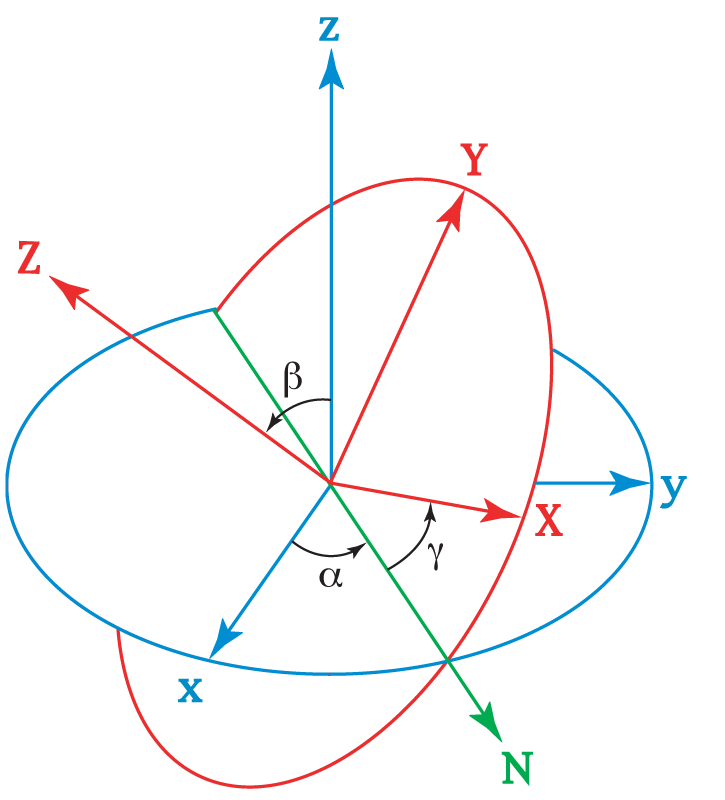
\includegraphics[width=8cm, height=8cm]{1.png}
 
 Рисунок 2.1 --- углы Эйлера
\end{center}

Получаем СЛАУ размерности $M+1:M+1$, которую можно решить с помощью пакета Scilab. 

\end{document}
